\documentclass[12pt]{article}
\usepackage{setspace}
\usepackage{fullpage}
\usepackage{textcomp}
\usepackage[utf8]{inputenc}
\usepackage{float}

\frenchspacing
\usepackage{indentfirst}

\usepackage{graphicx}
\DeclareGraphicsExtensions{.png}
\DeclareGraphicsExtensions{.jpg}

\usepackage[hidelinks]{hyperref}
\usepackage{url}

\newcommand{\nl}{\newline}

\begin{document}

\section*{Main Problem Statement}

We want you to write your own algorithm to generate a Voronoi Diagram. \nl

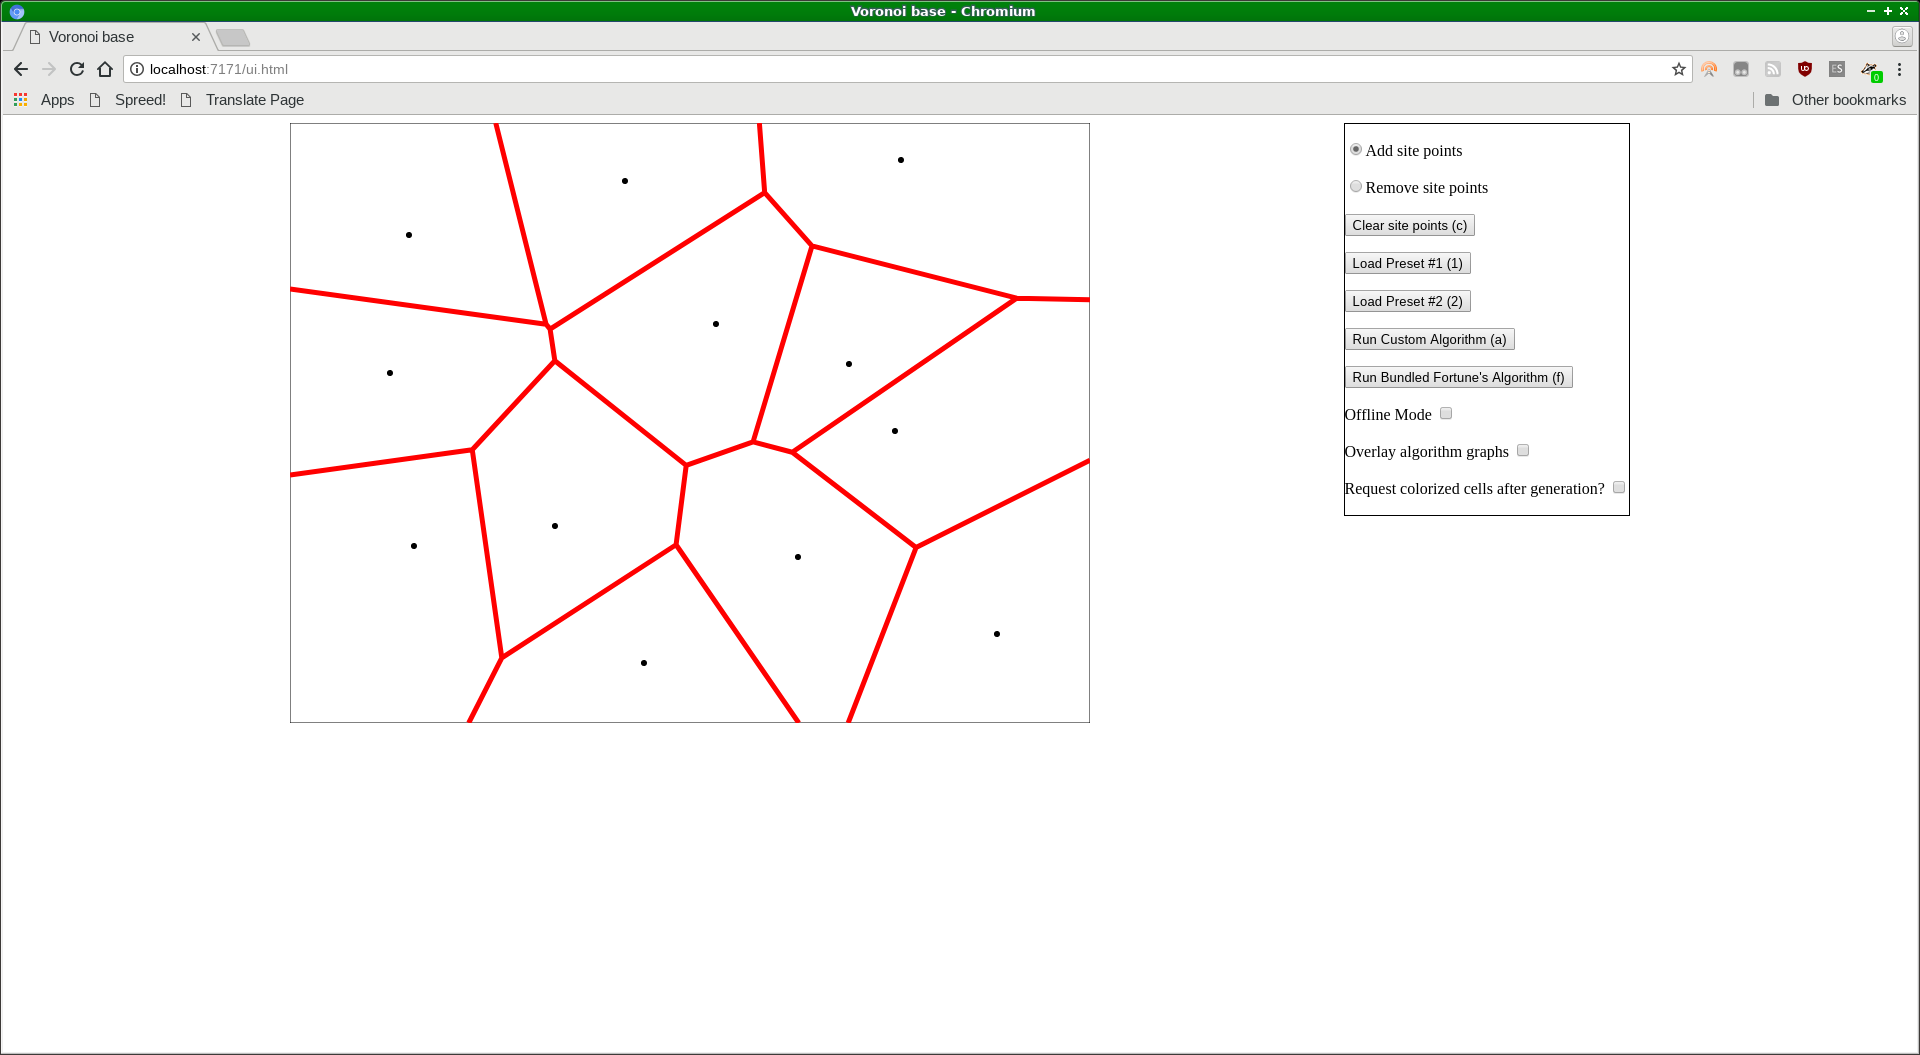
\includegraphics[width=0.99\textwidth]{screenshot_nocolor.png}

\subsection*{Background Info}

The above graphic shows a complete diagram. There are several dots in the
diagram -- these represent control points, or Sites. $n$ of these are inputted
arbitrarily by a user, you are guaranteed at least 2. The Voronoi ``diagram''
is the unique set of line segments (or pixels) that are red in the graph.

Around each Site point is a set of colored edges, or line segments, that define the Site's
Cell or polygon. The formal definition of the Voronoi diagram is such that for each
$(x, y)$ point within a Cell, the corresponding Site point is the closest (by
Euclidean distance) Site point. If two or more Site points are equidistant,
then that represents a boundary location for the Cells and is therefore
colored as part of a line in the diagram above.

Stating the same thing but more mathematically,\nl\nl
Site $S := (S_x, S_y)$ \nl
Sites $:= \exists \{S_i\}$, $2 \leq i \leq n$ \nl
Cell in site $:= \forall S_i \exists C_i$ \nl
Relationship of points $:= \forall (x,y) \in C_i$ and $\forall i \neq j
\rightarrow distBetween((x,y), S_i) \leq distBetween((x,y), S_j)$

\subsection*{Framework Details}

You should have received a README file with this project which covers how to
setup the project. If you have not gone through that yet, please do so now, then
come back to this document.

We've provided a framework in order to make your primary task as straightforward as
possible but also to support supplementary tasks as needed. From the README you
should have learned you can use either Java or JavaScript. If opting for Java,
you should have opened and launched \texttt{Application.java} and have \url{http://localhost:7171/ui.html}
open in a browser window. If opting for JavaScript instead, you just need to
open the \texttt{ui.html} file with the browser directly (most will open it if
you drag and drop).
% https://htmlpreview.github.io/?https://github.com/Jach/voronoi_base/blob/master/ui.html

Included is a known-correct implementation of Fortune's Algorithm, an
efficient method of generating these diagrams. (We do not expect you
to derive and write your own version of that algorithm; fortunately there are
many ways of generating these diagrams!) It will draw the diagram in red for
you to compare your own output against. You can toggle which algorithm to use
from the client.

The client front-end defines a bounding box rectangle 800x600 pixels and this
information is passed along to the code you will write, however the UI is resilient
to drawing out of bounds. For instance,
if you returned an edge from $(-400, -300)$ to $(1600,1200)$, you will still see
a visible line as if your edge was from $(0,0)$ to $(800,600)$.

\subsection*{Framework Details (Java)}

The Java file \texttt{CustomAlgorithm.java} in the package
\texttt{com.thejach.voronoi.custom} is the primary file you will need to edit in
order to complete the problem statement. You are of course free to introduce new
files (and tests) as you see fit. Open source dependencies are also allowed if
you think it appropriate, but note the intent is to see what you can do directly,
not just what other software you can manipulate.

You should open \texttt{CustomAlgorithm.java} now. It has a method \texttt{generate()}
whose role is to populate the object's \texttt{graph} variable with new \texttt{Edge} objects.
An Edge represents a line segment, with a start point $(x_0, y_0)$ and an end point
$(x_1, y_1)$.
The file contains further comments on the usage of the existing code.

%When the client requests graph generation, it will send up the set
%of Site points, and expect a set of edges in return. It will then draw the edges
%for you. If, however, your Edge consists of a start and end point that is the
%same, the client will draw a single pixel point for it. (Yes, this means you
%could generate the diagram with just a bunch of pixel ``edges''!)

\subsection*{Framework Details (JavaScript)}

The JS file \texttt{custom\_algorithm.js} is the primary file you will need to
edit in order to complete the problem statement, the area to edit is at the
bottom of the file.

Just like the Java version, there is a \texttt{generate} method
whose role is to add edge points. This is where you will write your code, but
you can add any other functions or methods you need. The file contains further
comments on the usage of the existing code.

\subsection*{Scoring Criteria}

Our intent is to keep any candidate busy for the allotted time, not to make a
single pass/fail type of problem. As such \textbf{there are many ways you can make a
positive impression, even if you can't complete the primary problem statement as
given.}
You should attempt the problem statement for maximum effect, but here are some
suggestions for other things you can do instead / in addition, and you're free
to try wowing us with your own ideas here.

\begin{enumerate}
  \item Try solving a simpler subproblem first; for example what is the diagram
    when you only have two Site points?\footnote{Some testing has shown that even this simpler subproblem can take
    good candidates over half an hour to make a clean and robust solution, so if you
    are considering this near the end, make sure you've paced yourself.} What about only 3 points? \textbf{Make
    sure you include any partial or incremental work even if it doesn't end up in the final code
    path!}
  \item The UI is robust to out-of-bounds edges, but what if it wasn't? Would
    your code work? Can you verify that it would work? Are there other edge
    cases?
  \item We are a dev/QE hybrid team. The provided \texttt{FortuneAlgorithm.java}
    class results in a known-correct set of edges, but is it actually correct?
    How might you assess its quality? Feel free to provide an optional commentary text
    file if you have anything interesting to say about the existing code or your
    own code.
  \item A dual graph of a Voronoi diagram is a Delaunay triangularization. Can
    you generate the dual? Can you output its edges so that it draws?
  \item Can you color the graph Cells such that no two adjacent cells share the
    same color, and so you never have to use more than the minimum necessary
    unique colors? (See \texttt{GraphColorizer.java} or
    \texttt{graph\_colorizer.js} for hints on where to start if you decide to
    try this.)
  \item If you generate the graph by plotting a bunch of points, can you take
    your set of points and construct a minimum set of edges that pass through
    all of them?
  \item How do other distance metrics besides Euclidean distance impact the
    graph?
  \item Is your code straightforward to follow?
  \item Do you understand the performance profile?
  \item If this is child's play, you can attempt your own version of Fortune's
    Algorithm, just be ready to explain it to us!
  \item Do you really hate Java/JS? Well, that's what we mostly do here! But
    you're free to write your own stuff from scratch in whatever language and
    stack you like (for instance an android app done in Kotlin), but it must
    allow us to interactively add points and generate a diagram.

\end{enumerate}

\subsection*{Potentially Useful Formulas}

\noindent
Distance formula for the distance between two points $(x_0, y_0)$ and $(x_1,
y_1)$:
$$distance = \sqrt{(x_0 - x_1)^2 + (y_0 - y_1)^2)}$$

\noindent\nl
Midpoint formula for the midpoint between two points:
$$(x_m, y_m) = (\frac{x_0+x_1}{2}, \frac{y_0+y_1}{2})$$

\noindent\nl
Formula of a line:
$$y = mx + b$$ 
where $m$ is the line slope, $b$ is the
y-intercept, and so given $x$ you can calculate $y$.

\noindent\nl
Alternate formula of a line:
$$y = m(x-a)+b$$
where $m$ is the line slope, and the
point $(a,b)$ is any known point on the line.

\noindent\nl
Slope between two points:
$$slope = \frac{\Delta y}{\Delta x} = \frac{y_1 - y_0}{x_1 - x_0}$$

\noindent\nl
Perpendicular slope:
$$slope_{perp} = \frac{-1}{slope}$$

If you need a refresher on how to represent and graph a line:
\url{https://www.youtube.com/watch?v=IL3UCuXrUzE}

This is open book / internet, just be prepared to deeply explain everything you
do including how you arrived at writing any particularly piece of code. Marking
commented out sections / otherwise dead code can be illuminating for our end in
understanding how you develop software.

\end{document}
